\newpage
\subsection{Caso d'uso UC9 - Acquisto API}
\label{UC9}
\begin{figure}[ht]
	\centering
	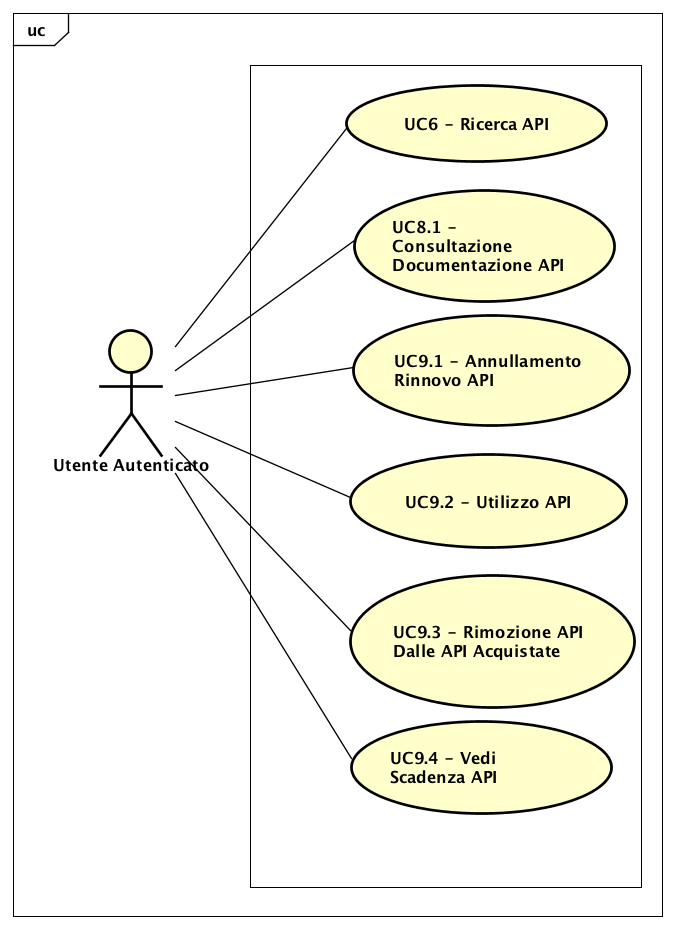
\includegraphics[scale=0.45]{UML/UC9.png}
	\caption{UC9: Acquisto API}
\end{figure}

\begin{longtable}{ l | p{11cm}}
	\hline
	\rowcolor{Gray}
	\multicolumn{2}{c}{UC9 - Acquisto API}\\
	\hline
	\textbf{Attori} & Utente autenticato, Amministratore API Market \\
	\textbf{Descrizione} & L'attore può effettuare l'acquisto dell'API selezionata tramite i crediti da lui posseduti \\
	\textbf{Pre-Condizioni} & L'attore ha selezionato una API e si trova nella relativa schermata di acquisto \\
	\textbf{Post-Condizioni} & L'attore ha acquistato l'API selezionata \\
	\textbf{Scenario Principale} & 
	\begin{enumerate*}[label=(\arabic*.),itemjoin={\newline}]
		\item L'attore può visualizzare il nome dell'API (UC7.1)
		\item L'attore può visualizzare l'autore dell'API (UC7.3)
		\item L'attore può scegliere la licenza API desiderata (UC9.1)
		\item L'attore può visualizzare il prezzo dell'API selezionata (UC7.8)
		\item L'attore può visualizzare il saldo disponibile nel suo conto virtuale (UC12.2.1)
		\item L'attore può ricaricare il proprio conto virtuale (UC12.2.2)
		\item L'attore può visualizzare il saldo preventivato in seguito all'acquisto della licenza selezionata (UC9.2)
		\item L'attore può confermare l'acquisto (UC9.3), venendo reindirizzato ad una schermata di riepilogo (UC9.4)
	\end{enumerate*}\\
	\textbf{Scenari Alternativi} & 
	\begin{enumerate*}[label=(\arabic*.),itemjoin={\newline}]
		\item L'attore può visualizzare un messaggio di errore e la transazione non avviene (UC9.5)
	\end{enumerate*}\\
\end{longtable}

\newpage
\subsubsection{Caso d'uso UC9.1: Scelta licenza API}
\label{UC9_1}
\begin{figure}[ht]
	\centering
	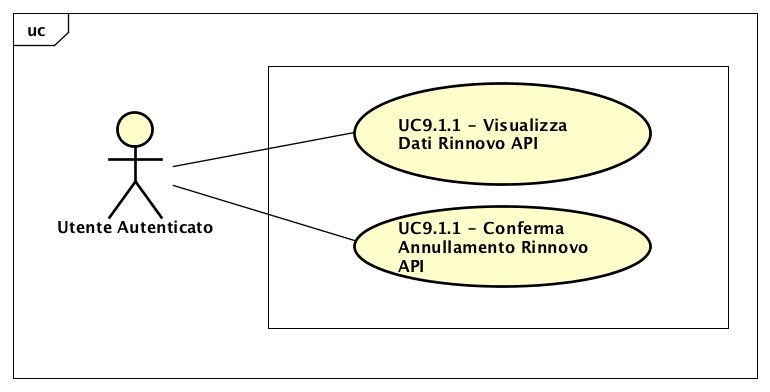
\includegraphics[scale=0.45]{UML/UC9_1.png}
	\caption{UC9.1: Scelta licenza API}
\end{figure}

\begin{minipage}{\linewidth}
	\begin{tabular}{ l | p{11cm}}
		\hline
		\rowcolor{Gray}
		\multicolumn{2}{c}{UC9.1 - Visualizzazione menù licenza} \\
		\hline
		\textbf{Attori} & Utente autenticato, Amministratore API Market \\
		\textbf{Descrizione} & L'attore sceglie tra le licenze quella desiderata, oppure lascia inalterata la scelta di default \\
		\textbf{Pre-Condizioni} & L'attore ha selezionato una API e si trova nella relativa schermata di acquisto \\
		\textbf{Post-Condizioni} & L'attore ha selezionato la licenza desiderata, oppure ha lasciato inalterata la scelta di default \\
		\textbf{Scenario Principale} & 
		\begin{enumerate*}[label=(\arabic*.),itemjoin={\newline}]
			\item L'attore può selezionare la licenza per numero di chiamate, impostata di default (UC9.1.1)
			\item L'attore può selezionare la licenza per tempo di utilizzo (UC9.1.2)
			\item L'attore può selezionare la licenza per traffico (UC9.1.3)
		\end{enumerate*}\\
	\end{tabular}
\end{minipage}

\paragraph{Caso d'uso UC9.1.1: Scelta licenza per numero di chiamate}
\label{UC9_1_1}

\begin{minipage}{\linewidth}
	\begin{tabular}{ l | p{11cm}}
		\hline
		\rowcolor{Gray}
		\multicolumn{2}{c}{UC9.1.1 - Scelta licenza per numero di chiamate} \\
		\hline
		\textbf{Attori} & Utente autenticato, Amministratore API Market \\
		\textbf{Descrizione} & L'attore sceglie la licenza API per numero di chiamate \\
		\textbf{Pre-Condizioni} & L'attore visualizza il menù per la scelta della licenza API  \\
		\textbf{Post-Condizioni} & L'attore ha scelto la licenza API per numero di chiamate \\
		\textbf{Scenario Principale} & 
		\begin{enumerate*}[label=(\arabic*.),itemjoin={\newline}]
			\item L'attore può scegliere la licenza API per numero di chiamate
		\end{enumerate*}\\
	\end{tabular}
\end{minipage}

\paragraph{Caso d'uso UC9.1.2: Scelta licenza per tempo di utilizzo}
\label{UC9_1_2}

\begin{minipage}{\linewidth}
	\begin{tabular}{ l | p{11cm}}
		\hline
		\rowcolor{Gray}
		\multicolumn{2}{c}{UC9.1.2 - Scelta licenza per tempo di utilizzo} \\
		\hline
		\textbf{Attori} & Utente autenticato, Amministratore API Market \\
		\textbf{Descrizione} & L'attore sceglie la licenza API per tempo di utilizzo \\
		\textbf{Pre-Condizioni} & L'attore visualizza il menù per la scelta della licenza API  \\
		\textbf{Post-Condizioni} & L'attore ha scelto la licenza API per tempo di utilizzo \\
		\textbf{Scenario Principale} & 
		\begin{enumerate*}[label=(\arabic*.),itemjoin={\newline}]
			\item L'attore può scegliere la licenza API per tempo di utilizzo
		\end{enumerate*}\\
	\end{tabular}
\end{minipage}

\paragraph{Caso d'uso UC9.1.3: Scelta licenza per traffico}
\label{UC9_1_3}

\begin{minipage}{\linewidth}
	\begin{tabular}{ l | p{11cm}}
		\hline
		\rowcolor{Gray}
		\multicolumn{2}{c}{UC9.1.3 - Scelta licenza per traffico} \\
		\hline
		\textbf{Attori} & Utente autenticato, Amministratore API Market \\
		\textbf{Descrizione} & L'attore sceglie la licenza API per traffico \\
		\textbf{Pre-Condizioni} & L'attore visualizza il menù per la scelta della licenza API  \\
		\textbf{Post-Condizioni} & L'attore ha scelto la licenza API per traffico \\
		\textbf{Scenario Principale} & 
		\begin{enumerate*}[label=(\arabic*.),itemjoin={\newline}]
			\item L'attore può scegliere la licenza API per traffico
		\end{enumerate*}\\
	\end{tabular}
\end{minipage}

\subsubsection{Caso d'uso UC9.2: Visualizzazione previsione saldo finale}
\label{UC9_2}

\begin{minipage}{\linewidth}
	\begin{tabular}{ l | p{11cm}}
		\hline
		\rowcolor{Gray}
		\multicolumn{2}{c}{UC9.2 - Visualizzazione previsione saldo finale} \\
		\hline
		\textbf{Attori} & Utente autenticato, Amministratore API Market \\
		\textbf{Descrizione} & L'attore visualizza una previsione del proprio saldo crediti in seguito all'acquisto\\
		\textbf{Pre-Condizioni} & L'attore ha selezionato una API e si trova nella relativa schermata di acquisto \\
		\textbf{Post-Condizioni} & L'attore ha visualizzato una previsione del proprio saldo in seguito all'acquisto \\
		\textbf{Scenario Principale} & 
		\begin{enumerate*}[label=(\arabic*.),itemjoin={\newline}]
			\item L'attore può visualizzare una previsione del proprio saldo finale qualora acquistasse l'API con la licenza scelta in UC9.1
		\end{enumerate*}\\
	\end{tabular}
\end{minipage}

\subsubsection{Caso d'uso UC9.3: Conferma acquisto API}
\label{UC9_3}

\begin{minipage}{\linewidth}
	\begin{tabular}{ l | p{11cm}}
		\hline
		\rowcolor{Gray}
		\multicolumn{2}{c}{UC9.3 - Conferma acquisto API} \\
		\hline
		\textbf{Attori} & Utente autenticato, Amministratore API Market \\
		\textbf{Descrizione} & L'attore può confermare l'acquisto dell'API, portando a termine la transazione, ricevendo un'email di riepilogo e visualizzando una schermata di riepilogo dell'acquisto appena realizzato \\
		\textbf{Pre-Condizioni} & L'attore ha selezionato una API e si trova nella relativa schermata di acquisto \\
		\textbf{Post-Condizioni} & L'attore ha confermato l'acquisto dell'API \\
		\textbf{Scenario Principale} & 
		\begin{enumerate*}[label=(\arabic*.),itemjoin={\newline}]
			\item L'attore può confermare l'acquisto dell'API, portando a termine la transazione, ricevendo un'email di riepilogo e visualizzando una schermata di riepilogo dell'acquisto appena realizzato (UC9.4)
		\end{enumerate*}\\
	\end{tabular}
\end{minipage}

\subsubsection{Caso d'uso UC9.4: Riepilogo acquisto API}
\label{UC9_4}

\begin{minipage}{\linewidth}
	\begin{tabular}{ l | p{11cm}}
		\hline
		\rowcolor{Gray}
		\multicolumn{2}{c}{UC9.4 - Riepilogo acquisto API} \\
		\hline
		\textbf{Attori} & Utente autenticato, Amministratore API Market \\
		\textbf{Descrizione} & L'attore conferma l'acquisto dell'API, portando a termine la transazione e visualizzando un messaggio di ringraziamento \\
		\textbf{Pre-Condizioni} & L'attore ha confermato l'acquisto per l'API \\
		\textbf{Post-Condizioni} & L'attore ha visualizzato il riepilogo dell'acquisto appena realizzato \\
		\textbf{Scenario Principale} & 
		\begin{enumerate*}[label=(\arabic*.),itemjoin={\newline}]
			\item L'attore può visualizzare un messaggio di ringraziamento (UC9.4.1)
			\item L'attore può visualizzare il nome dell'API appena acquistata (UC7.1)
			\item L'attore può visualizzare la chiave dell'API appena acquistata (UC7.9)
		\end{enumerate*}\\
	\end{tabular}
\end{minipage}

\paragraph{Caso d'uso UC9.5: Errore acquisto API}
\label{UC9_5}

\begin{minipage}{\linewidth}
	\begin{tabular}{ l | p{11cm}}
		\hline
		\rowcolor{Gray}
		\multicolumn{2}{c}{UC9.5 - Errore acquisto API} \\
		\hline
		\textbf{Attori} & Utente autenticato, Amministratore API Market \\
		\textbf{Descrizione} & L'attore visualizza un messaggio di errore e la transazione non avviene \\
		\textbf{Pre-Condizioni} & L'attore ha confermato l'acquisto per una API ma si è verificato un errore \\
		\textbf{Post-Condizioni} & L'attore ha visualizzato un errore relativo all'acquisto, con opportuna descrizione \\
		\textbf{Scenario Principale} & 
		\begin{enumerate*}[label=(\arabic*.),itemjoin={\newline}]
			\item L'attore può visualizzare un messaggio di errore e la transazione non avviene (E.g: L'API è in fase di cancellazione)
		\end{enumerate*}\\
	\end{tabular}
\end{minipage}